Wir haben für die Aufnahme der Signale viel verschiedene Situationen ausgesucht, um ein möglichst breites Spektrum an Raum-Effekten zu erhalten. Aufnahmeorte waren beispielsweise der Platz vor dem HSZ, die Wiese zwischen Physik- und Mathematikgebäude, sowie der Trefftzbau. Außerdem wurde in einer Wohnung gemessen, um Effekte von schallabsorbierenden Stoffen wie Teppich oder Bett zu erhalten. Soweit möglich, haben wir die natürliche Geräuschkulisse am jeweiligen Ort eingefangen. Zusätzlich dazu wurde ein definiertes Signal mittels eines Lautsprechers erzeugt, um Direktschall zu nutzen. Bei diesen Aufnahmen sollten die Effekte des Raumes am deutlichsten hervortreten.
\subsection{Beispielsignale}
\subsubsection{Signal 1 - trefftz$\_$wiese$\_$m}
\begin{figure}[ht!]
  \centering
  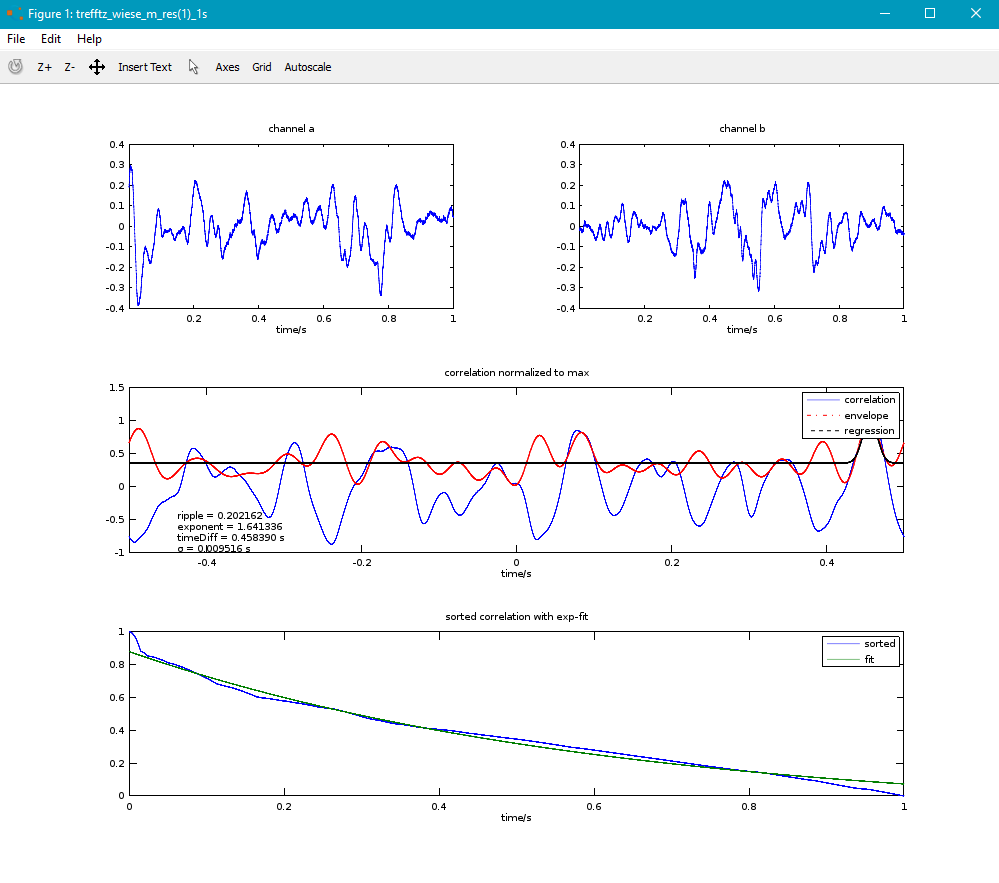
\includegraphics[scale=0.6]{img/trefftz_wiese_m}
  \caption{Signal 1}
  \label{figure2}
\end{figure}
\begin{figure}[ht!]
  \centering
  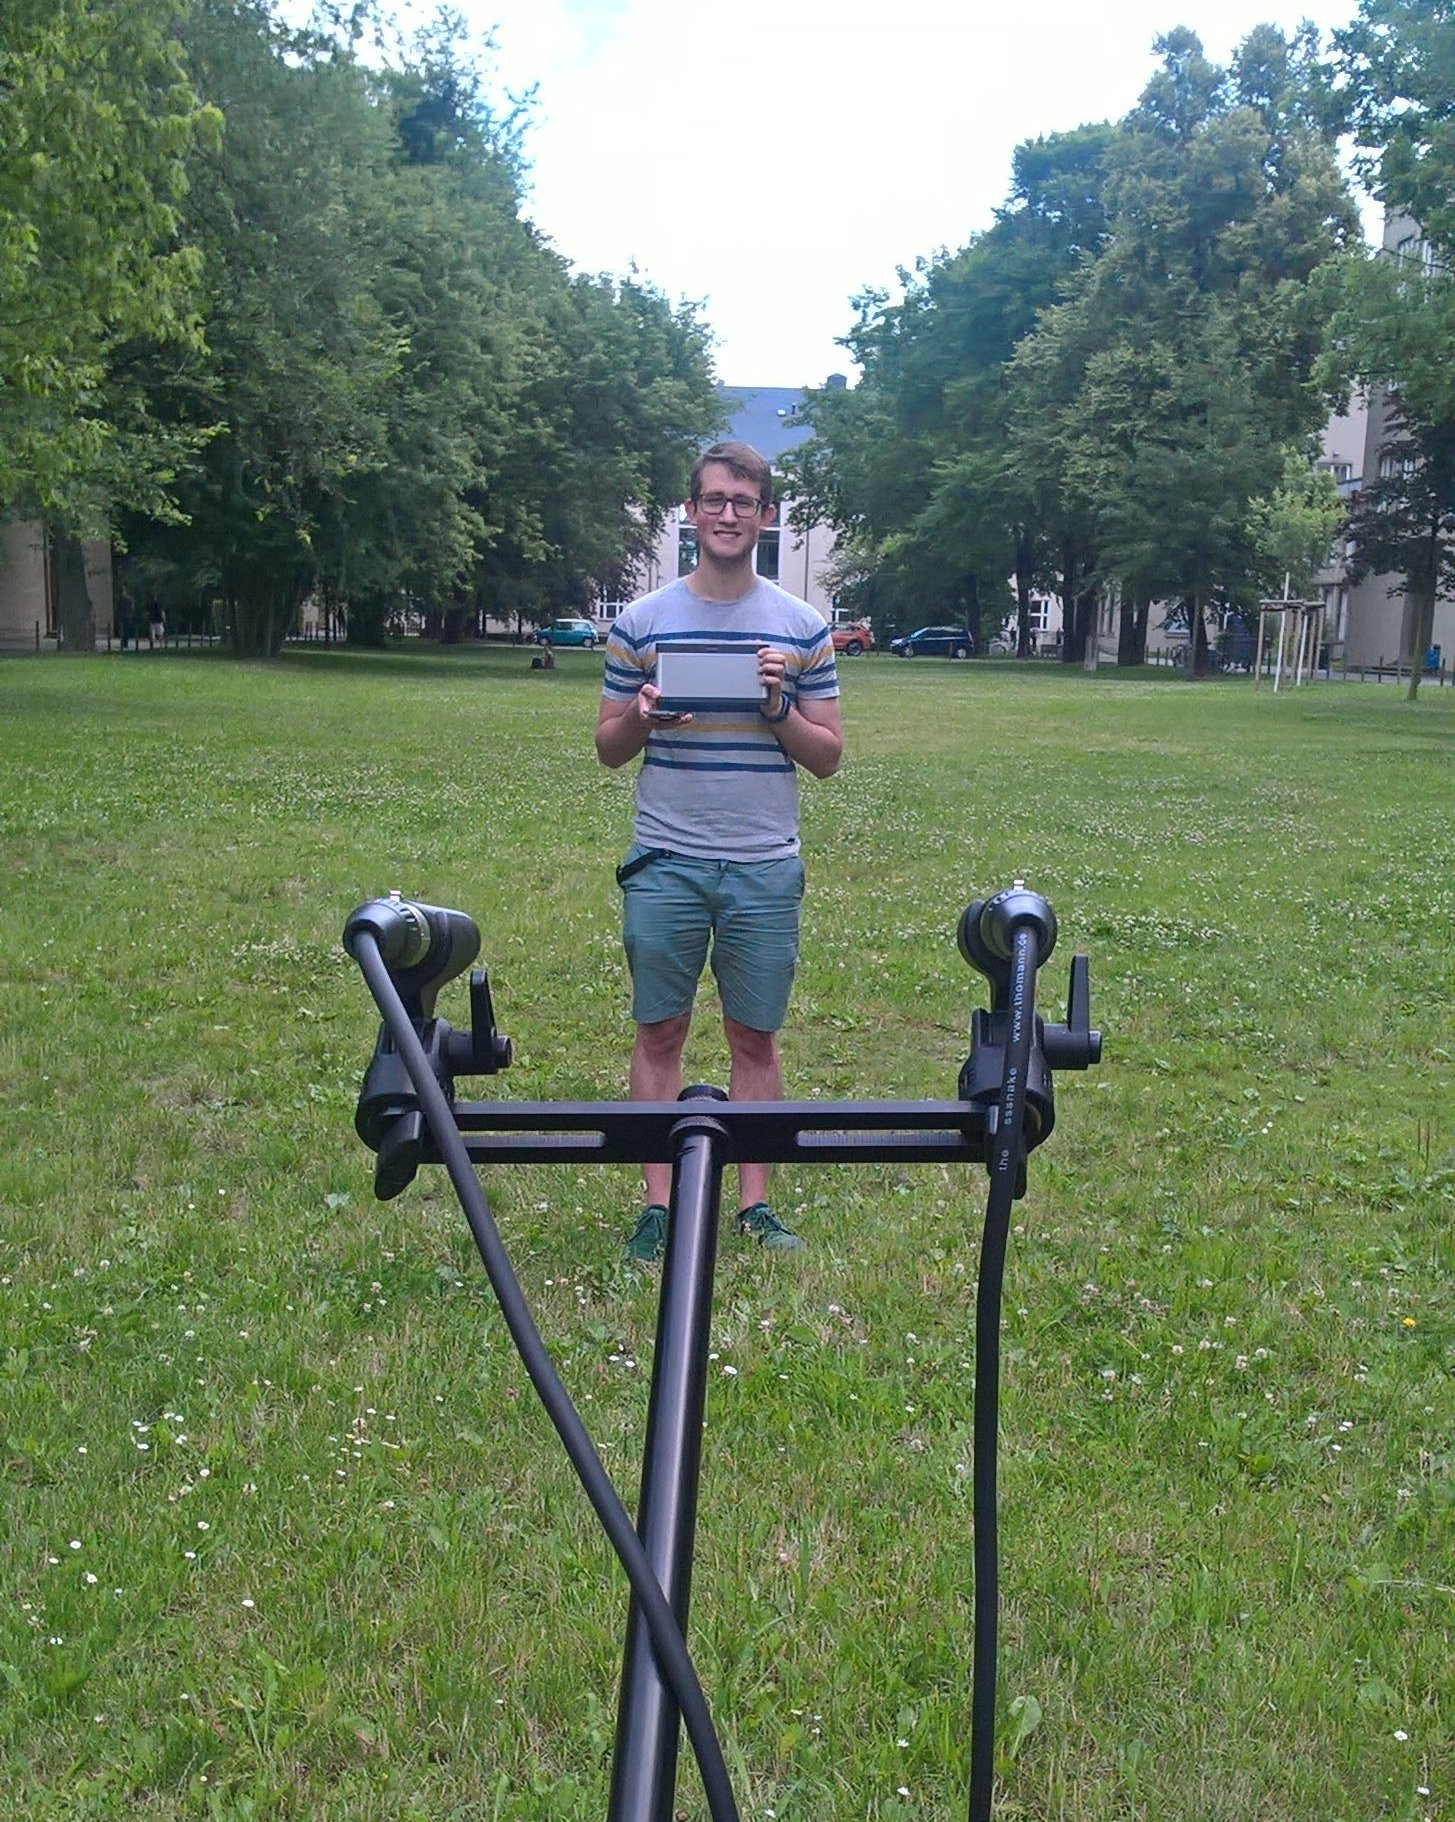
\includegraphics[width=0.4\textwidth]{img/wiese}
  \caption{Aufnahmesituation auf der Wiese des Trefftzbaus}
  \label{figure4}
\end{figure}
\paragraph{Aufnahmesituation} Dieses Signal wurde auf der Wiese zwischen dem Gebäude der Mathematik- und Physikfakultät aufgenommen. Dies stellt eine relativ große Freifläche mit wenigen Hindernissen mit ungehinderter Schallausbreitung dar, wobei jedoch auch die umliegenden Gebäude einen Einfluss auf das Ausbreitungsverhalten haben können. Es wurde eine zusätzliche Primärschallquelle genutzt, die während der Aufnahme stationär an einem Punkt im Raum blieb. Dieser Punkt befand sich frontal zu den Mikrofonen in einigen Metern Abstand. Durch diese Anordnung sollte zum einen ein definiertes Signal vorgegeben, aber zum anderen auch der Effekt der Umgebung erfasst werden. 
Um den Einfluss einer bewegten Schallquelle zu untersuchen, führten wir bei ähnlichem Messaufbau auch noch eine Messung durch in der wir die Primärschallquelle senkrecht zur Ausrichtung der Mikrofone bewegten. Die Ergebnisse dieser Messung sind im Anhang zu finden.
\paragraph{Signalbeschreibung} Wie in Abbildung \ref{figure2} zu sehen ist, ändern sich beide Kanäle relativ langsam. Sowohl Kanal A als auch Kanal B sind klar definiert und im Vergleich zum Rauschen relativ groß. Man erkennt jedoch bereits beim einfachen Betrachten, dass sich beide Seiten nur sehr geringfügig ähnlich sehen.
\paragraph{Beschreibung der KKF} Die Kreuzkorrelationsfunktion schwankt sehr stark über den gesamtem Zeitbereich. Deswegen ist auch die Hüllkurve stark schwankend. Da die Regression über die Hüllkurve berechnet wird, wird diese dem Signal auch nicht gerecht.
\paragraph{Auswertung der Maßzahlen}
Der ripple-Faktor von Signal 1 ist mit einem Wert von 0.2 vergleichsweise niedrig. Dass nur ein geringer Anteil der Energie des Signals in den obersten 5 Prozent der Werte vorhanden ist, lässt sich auch gut an der KKF erkennen. Es gibt nur sehr wenige Peaks. Die Aussagekräftigkeit von $\sigma$ ist hier sehr gering. Wie gut zu erkennen ist, hat die Kurve keine Ähnlichkeit mit einer Gauß-Glocke. Auch die anderen Werte sind für dieses Signal schwierig zu bewerten, da die Ähnlichkeit generell sehr klein ist.
\subsubsection{Signal 2 - trefftz$\_$fahrstuhl$\_$m}
\begin{figure}[ht!]
  \centering
  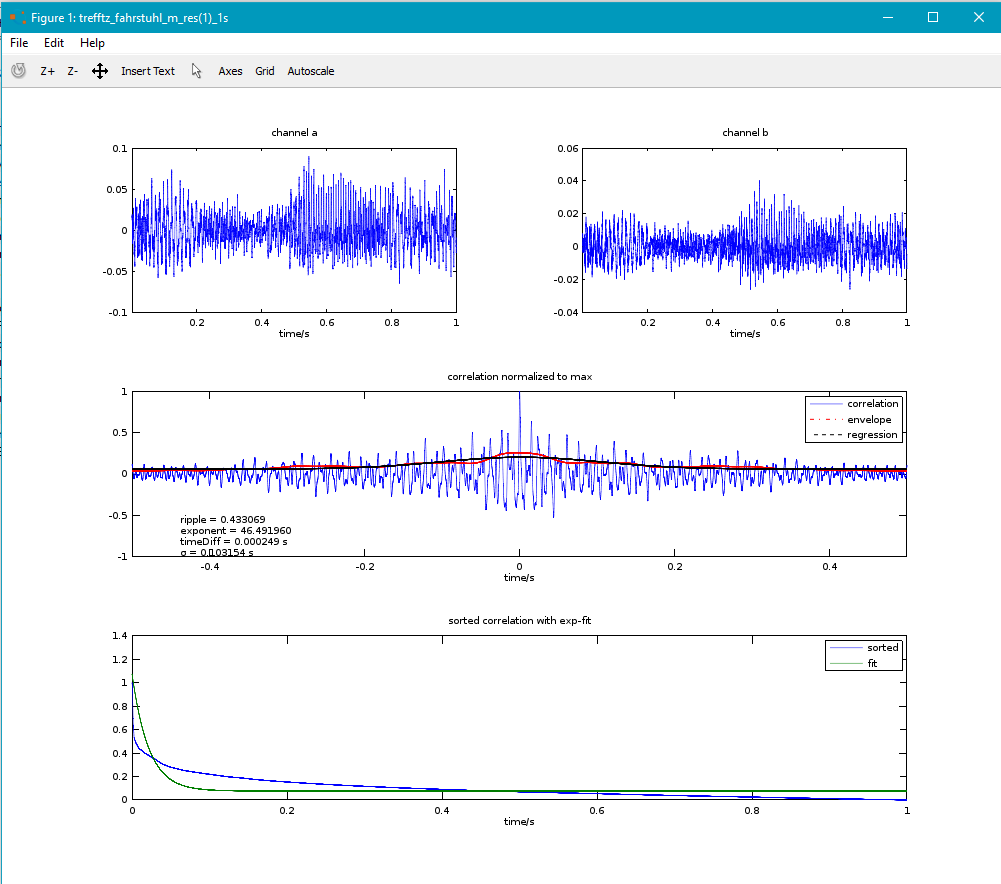
\includegraphics[scale=0.6]{img/trefftz_fahrstuhl_m}
  \caption{Signal 2}
  \label{figure3}
\end{figure}
\begin{figure}[ht!]
  \centering
  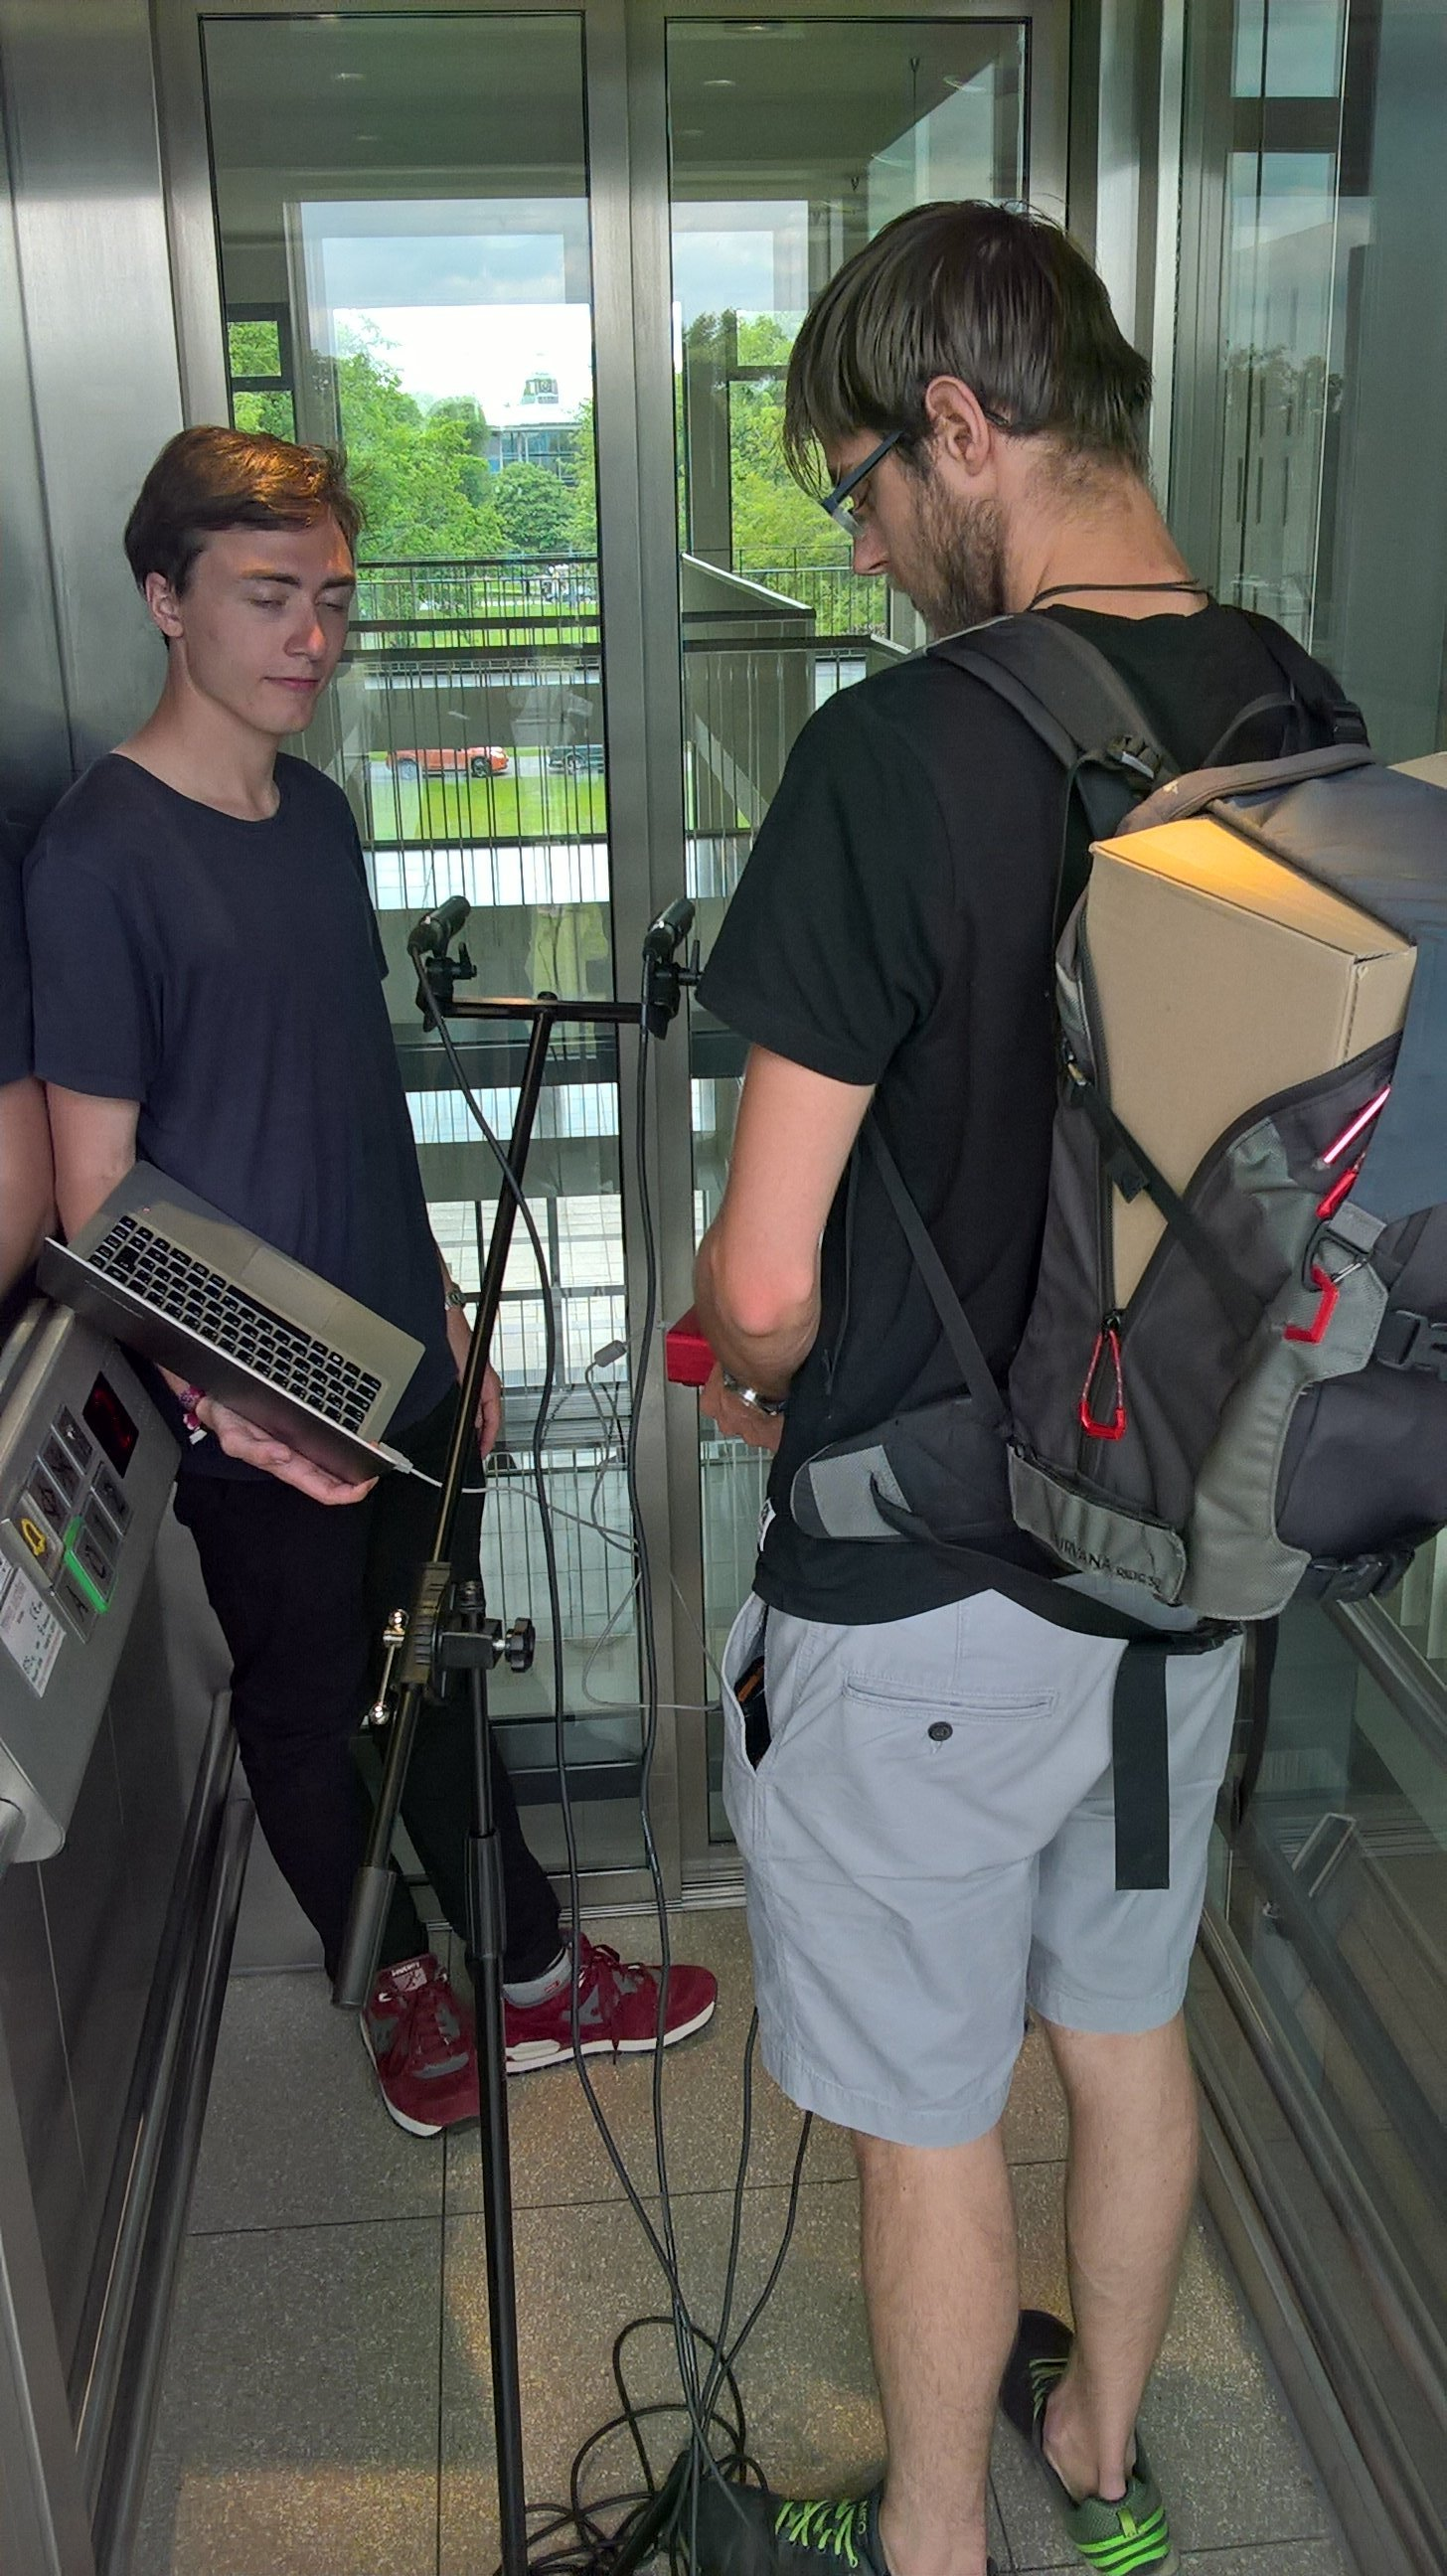
\includegraphics[width=0.4\textwidth]{img/fahrstuhl}
  \caption{Aufnahmesituation im Fahrstuhl des Trefftzbaus}
  \label{figure5}
\end{figure}

\paragraph{Aufnahemsituation} Diese Aufnahme fand im Fahrstuhl des Trefftzbaus statt. Das heißt, dass der Raum war relativ klein und ist mit dicken Glaswänden versehen. Um ein Signal zu erhalten wurde eine Primärschallquelle in Form eines hochwertigen Lautsprechers genutzt über den ein Beispielsignal wiedergegeben wurde. Da der Raum im Fahrstuhl sehr begrenzt war, ließen sich unterschiedliche Messaufbauten schwer realisieren und auch eine Bewegung der Primärschallquelle war nicht möglich. Weiterhin sei erwähnt, dass wir uns während der Messung im Fahrstuhl befanden und somit nicht nur der Raum allein vermessen wurde. Da gerade das aber eine reale Situation im Fahrstuhl ausmacht, hat dies keine negativen Auswirkungen auf die Aussagekraft des Signals. 
\paragraph{Signalbeschreibung}
In Abbildung \ref{figure3}  erkennt man sehr gut, dass sich beide Kanäle sehr schnell ändern und einen ähnlichen Verlauf haben. Lediglich die Lautstärke des Signals ist unterschiedlich. Das stört jedoch nicht für die Berechnung der Maßzahlen, da diese nicht von der Amplitude  abhängig sind. 
\paragraph{Beschreibung der KKF}
Für dieses Signal ist auch an der Kreuzkorrelationsfunktion klar zu sehen, dass es ein Maximum in der Mitte gibt. Das heißt, die Signale sind sich sehr ähnlich. Zu den Seiten nimmt die KKF langsam ab. Für solch einen Verlauf ist die Aussage der Hüllkurve und der Regression sehr gut, da diese Kreuzkorrelation gut mit einer Gauß-Kurve approxmiert werden kann.
\paragraph{Auswertung der Maßzahlen}
Der ripple-Faktor liegt mit 0.43 recht hoch, das heißt ein großer Teil der Signal-Energie liegt innerhalb des fünften Percentils. Die Aussage des Gauß-Fits ist hier wesentlich besser als bei Signal 1. Dies kann man gut in der Abbildung \ref{figure3} erkennen, denn der Verlauf der Hüllkurve kommt der Form einer Gauß-Glocke recht nah. Die Zeitverschiebung des Maximums der KKF ist minimal. Daran ist zu erkennen, dass das Signal an beiden Mikrofonen nur mit sehr kleiner Verzögerung angekommen ist, was im begrenzen Raum des Fahrstuhl auch Sinn ergibt.

\subsection{Probleme bei der Signalauswahl}
Bei der Signalauswahl ergab sich das Problem, dass man möglichst viele verschiedene Raumsituationen erfassen musste, um eine große Menge verschiedener Daten zu bekommen. Dabei war es jedoch nur schwer möglich vor Ort zu entscheiden, ob die entsprechende Aufnahme sinnvolle Ergebnisse liefert.
In den meisten Situationen war der Lautstärkepegel im Raum zu gering um 20s aufzunehmen, ohne das der Großteil der Aufnahme aus Rauschen bestand. Aus diesem Grund haben wir ein zusätzliches Signal erzeugt. Dadurch gibt es jedoch in den meisten Aufnahmen eine Primärquelle, die das Spektrum maßgeblich bestimmt.

\subsection{Fazit}
Abschließend lässt sich feststellen, dass der Gauß-Fit erst ab einem ripple-Faktor von 0.3 sinnvolle Ergebnisse liefert. Bei Werten die kleiner als 0.3 sind, ist die Hüllkurve einer Gauß-Kurve zu unähnlich. Es ist jedoch festzustellen, dass die Regression der Exponentialfunktion mit kleiner werdendem ripple besser über der nach Größe sortierten Amplituden liegt.
Es ist empfehlenswert, Signale in Räumen aufzunehmen, die ausreichend klein sind, damit die Raumeffekte Auswirkungen auf das Signal haben. Sonst nimmt man größtenteils rauschen auf, welches sehr geringe Aussagen zulässt.
